% !TEX TS-program = lualatex
\documentclass[titlepage]{article}
\usepackage[a5paper,margin=0.5in]{geometry}

%% Force using more of the margins than default
%\setlength{\oddsidemargin}{0.1in}
%\setlength{\evensidemargin}{0.1in}
%\setlength{\textwidth}{6.5in}
%\setlength{\topmargin}{0in}
%\setlength{\textheight}{8.5in}

%% Header
\usepackage{fancyhdr,lastpage}
\usepackage[mmddyyyy]{datetime}
\renewcommand{\dateseparator}{/}
\fancypagestyle{plain}{
    \fancyhf{} %Clear Everything.
    \lhead{ VisLang Final Report }
    \rhead{ Page \thepage\ of \pageref{LastPage} }
    \setlength{\headheight}{24pt}
    \setlength{\footskip}{24pt}
    \renewcommand{\headrulewidth}{1pt} %0pt for no rule, 2pt thicker etc...
    \renewcommand{\footrulewidth}{0pt}
}
\pagestyle{plain}
\usepackage{indentfirst}

%% Tables 
\usepackage{longtable}
\newcommand{\specialcell}[2][l]{%
      \begin{tabular}[#1]{@{}c@{}}#2\end{tabular}
}

%% Figures
\usepackage{wrapfig}

%% Items
\usepackage{enumitem}

%% Code Listings
\usepackage{minted}
\usepackage{listings}
\usepackage{color} % for colored solution
%\usepackage[svgnames]{xcolor}
\usepackage{caption}

% Custom macro for code listings from files
% #1 - language e.g. ocaml
% #2 - filename e.g. ../src/vislang.ml
% #3 - label e.g. src/top
% #4 - description e.g. Top Level
% note: filename will be pretty printed as vislang/src/*
%       instead of ../src/*
\newcommand{\srccode}[4]{
    \inputminted[frame=single,linenos,fontsize=\footnotesize]{#1}{#2}
    \captionof{listing}{\label{#3}#4: #2}
    \pagebreak
}

%% Diagrams
\usepackage{tikz}
\usetikzlibrary{shapes,arrows}
\tikzset{
    block/.style = {draw, 
                    rectangle, 
                    minimum height=2em, 
                    minimum width=12em,
                    node distance=1.5cm
    }
}

% Custom language for XML
\definecolor{maroon}{rgb}{0.5,0,0}
\definecolor{darkgreen}{rgb}{0,0.5,0}
\lstdefinelanguage{XML}
{
    basicstyle=\ttfamily\footnotesize,
    morestring=[b]",
    moredelim=[s][\bfseries\color{maroon}]{<}{\ },
    moredelim=[s][\bfseries\color{maroon}]{</}{>},
    moredelim=[l][\bfseries\color{maroon}]{/>},
    moredelim=[l][\bfseries\color{maroon}]{>},
    morecomment=[s]{<?}{?>},
    morecomment=[s]{<!--}{-->},
    commentstyle=\color{darkgreen},
    stringstyle=\color{blue},
    identifierstyle=\color{red}
    %morekeywords={name,type,scope,address,value,to,from,
    %              initial\_condition,reference}
}
\lstset
{
    language=XML,
    basicstyle=\footnotesize\ttfamily,
    tabsize=4,
    keepspaces=false,
    keywordstyle=\color{red},
    identifierstyle=\color{blue},
    commentstyle=\color{green},
    frame=single,
    captionpos=t%, % sets the caption-position to top
    %morestring=[s]{"}{"},
    %morecomment=[s]{!--}{--},
    %morekeywords={name,type,scope,address,value,to,from,
    %              initial\_condition,reference}
}

\newcommand{\includecode}[1]{\lstinputlisting[caption=#1]{#1}}

% For title page
\title{VisLang: A Visual Language\\Final Report}
\author{Bryant Eisenbach (UNI: bje2113)}
\date{Date: \today}

\begin{document}
% This command creates a title page
\maketitle
\pagebreak

\tableofcontents
\pagebreak

\listoffigures
\pagebreak

\listoftables
\pagebreak

\listoflistings
\pagebreak

% TODO
\section{Introduction}

VisLang is a block diagram language designed to allow fast and
easy prototyping of programs for embedded processors. The language is created
with a graphical editor in mind, and the core language is designed to be extensible
so that any graphical editor can add additional elements or attributes for graphical
display or other features.

\subsection{Key Language Features}

The language itself is based on the idea of blocks: small parts that can be grouped
together into ever larger blocks and re-used across different programs. VisLang has a
small group of fundamental (or atomic) blocks that will be understood by the VisLang
compiler. Other blocks will be constructed as groupings of these atomic blocks, and can
be referenced in other files. Libraries of useful function blocks can be constructed
from these atomic blocks containing common parts such as timers, latches, etc. The 
ability to include libraries and other blocks is a standard feature of the language.

The syntax of VisLang leverages standard XML, giving the language a well-formed and 
machine readable backbone. As noted previously, the point of leveraging XML is so that
3rd party programs can manipulate the file format in an easy way, and so that external
programs can add additional elements (e.g. visual information for display) and attributes
(e.g. location information) to the existing set of elements and attributes defined by
the language. Those tags (including XML comment tags) not included in the list of
recognized elements/attributes will be ignored by the compiler as a valid program is only
defined as a series of well-connected blocks. All parts require their necessary
attributes, and all connections require the source to exist. This creates a natural
flow to interpreting the language, such that any errors should be raised by the compiler
during compilation.

\subsection{Code Generation}

The VisLang Compiler will parse all of the parts specified in the input file and generate
a C source file that can be used in combination with other generated and manually created
C source files to generate fully functional programs for embedded devices. Each generated
file contains code that is completely reusable as the code generated has standard interfaces
and does not rely on global definitions.

\pagebreak

\section{Language Tutorial}

Any well-formed VisLang program can be constructed with the following guidance. Firstly,
the outer-most set of tags (the top of the XML tree or Top Block) must be a BLOCK element
and should be given a name appropiate to the intended functionality (file name and block
name do not have to match). Next, a selection of INPUT and OUTPUT elements should be chosen
for that block that describe how it will interface with other blocks or C source files.
When those have been chosen and given names and datatypes, it is now time to design the
inner logic of the block being made.
\par
Any collection of parts can be strung together
from any input to any output. The first important caveat to this is that the datatype
of each input and output must match to the corresponding connection being made. All parts
in VisLang have an explicit or implicit datatype, and that must be matched up as suggested
to avoid compilation errors. The second important caveat is that all calculations avoid
referencing themselves. This means that when tracing from any output to any input, there
is no instance of a calculation being used to define itself unless a MEM block has been
placed to prevent an algebraic loop occurance.
\par
Next comes the decision if there will be any references to external blocks.
The user can specify the location of an external block in a file using the following syntax:
"/path/to/file.vl$\vert$path$\vert$to$\vert$block". When using external blocks, it is
important to match the names and datatypes of the inputs/outputs to that block when
making connections to that block. Any incorrect types or names will be flagged as an error
at compilation time. Any BLOCK in any VisLang file can be referenced, but each file
must be compiled separately to avoid runtime errors when attempting to compile the target
generated C files.
\par
Finally, the design of the program could have grown to sufficient complexity where
encapsulating that functionality into a separate block would be desireable. At that point,
encapsulating all of the chosen parts into another BLOCK part would allow that part to
be isolated from other parts in the program (different namespace), and that part can be
referenced into another block in that program or any other.
\par
There are a few specific things about some of the parts VisLang provides worth noting.
All of the logic gate elements besides the NOT gate (AND, OR, etc.) and the SUMMER and
PROD elements are defined as having two or more inputs. The way this works in practice
is that each successive input increments the number after the word "input" e.g. "input1",
"input2", "input3", etc. when making connections to these parts. If a number is skipped
or the count does not start at 1, a compilation error will be raised. These parts are
known as "binary recursive" parts because the operation involved will be applied to every
input to the block in a recursive fashion e.g. (input1 op (input2 op (...))).
\par
Most attributes for elements are defined with a string. The name attribute is common to
every part in the VisLang language. The connection elements can reference these names
when making connections between any two blocks. If an element is an atomic part (any
element besides BLOCK and REFERENCE), then linking a block input to that name is as easy
as using that block's name. This is due to the fact that all of the atomic parts in VisLang
are defined as only having one output, so there is no ambiguity. The other attributes have
more explicit values that must match what is specified in the LRM.
\par
When using the "ic" or "value" attributes, values they require are literals of the relevant
datatype. Examples of literals for all VisLang types are below:
\begin{longtable}[c]{ |c|c| } 
    \hline
    datatype & example literal(s) \\ 
    \hline\hline
    boolean & false, true \\
    single, double & 1.000, -100., .000 \\
    integer & 100, 0x20, 2x1011, 8x671, -120 \\ 
    \hline
\end{longtable}

Note booleans can only be false or true. Floating point quantities (single, double) can
be a decimal quantity (with or without significant digits after the decimal point),
or specified using a decimal point e.g. 10.600. Floating point literals can also be
specified with a negative sign as well e.g. -1234.00. Integer quantities (e.g.
uint8, uint16, uint32, uint64, int8, int16, int32, int64) can be specified as a
decimal quantity (cannot have a decimal point), or using hex (e.g. 0x1A), binary
(e.g.2x1010), or octal (e.g. 8x2462) representation. Only signed integer datatypes can
have a negative sign in front.

\subsection{Example Program}

The following program illustrates some of the major features of the language. The
program itself takes an Input (presumably on the target device) and starts a
timer when the input is enabled. When the timer counts up to the target time, it
will set the Output true and reset the timer, creating a pulse-blinking light
with a period of 2 seconds.

\srccode{xml}{../example/timed-blinking-light.vl}{example:top}{Example Top Level}

As noted, the above file contained a reference to another part called timer defined
in timer.vs in the same directory. Any references must take place on a relative path
to that file, and that reference must contain the same number of inputs specified by
the target file inside the file referencing that part. The number of outputs need
not match, but any outputs specified in the file referencing that part must also
match what is available from the target file or an exception will be thrown. All
other unused outputs will be disregarded. The following file displays the target
file, complete with the relevant inputs and outputs as specified/required by the
previous file.

\srccode{xml}{../example/timer.vl}{example:timer}{Example Referenced Block}

\pagebreak

primatives: gates, memory/unit-delay blocks, I/O addresses (physical or virtual), switches, constants, timer, clock signal, library include statement, summer block, unary gain, multiplication/division, bitwise operator?

\pagebreak

% TODO
\section{Project Plan}

\subsection{Software Development Environment}

Development for the project took place entirely on an Asus Chromebook C720 using crouton
to enable a full linux environment. The tools used for this project are listed below:

\begin{itemize}
\item linux 3.10.18
\item ubuntu 14.04.2 LTS
\item git 1.9.1
\item vim 7.4.52
\item ocaml 4.01.0 (including ocamlyacc and ocamllex)
\item gcc 4.8.2
\item python 2.7.6
\end{itemize}

\subsection{Project Timeline}

% figure out timeline

\subsection{Project Log}
\srccode{pypylog}{../git.log}{prj:log}{Project Log}

\pagebreak

\section{VisLang Compiler Architecture}

\begin{wrapfigure}[25]{r}[-1.2cm]{0.25\textwidth}
  \centering
  \begin{tikzpicture}[auto]
    \node [block]                   (source)  {Source File (XML)};
    \node [block,below of=source]   (xmltok)  {XML Tokens};
    \node [block,below of=xmltok]   (xmlobj)  {XML Object Tree};
    \node [block,below of=xmlobj]   (blkobj)  {Block Object Tree};
    \node [block,below of=blkobj]   (optblk)  {Optimized Block Tree};
    \node [block,below of=optblk]   (gencod)  {Auto-generated Code};

    \draw[->] (source) -- node{xscanner.mll}    (xmltok);
    \draw[->] (xmltok) -- node{xparser.mly}     (xmlobj);
    \draw[->] (xmlobj) -- node{blockify.ml}     (blkobj);
    \draw[->] (blkobj) -- node{blockparse.ml}   (optblk);
    \draw[->] (optblk) -- node{compile.ml}      (gencod);
  \end{tikzpicture}
  \caption{VLCC Architecture}
  \label{arch:vlcc}
\end{wrapfigure}

The architecture of VisLang has two distinct stages of operation from source file to
target file. The scanning and parsing stages of the front end essentially implement
read the XML elements of interest and skip through parsing any unrecognized tokens.
After a correctly formed XML Object Tree has been formed, the next step is to translate
that tree of XML Objects (an XML Object has a tag, a list of attributes and a list of
inner objects, if any) into a block tree where each block can verify and access the
necessary attributes it should have. Each object can also see the list of connections
assigned to it when it was parsed, which is important when verifying the program is
well-formed. That block tree is then taken and re-organized such that the inner objects
of a block are in Static Single Assignment form, e.g. each block can be computed using
the outputs of previous blocks in the list for that containing block.
\par
In the process of reorganizing the inner blocks, the Block Parse algorithm will also
perform the check that the inner blocks align (e.g. they call blocks that are properly
assigned, they match in datatype, etc.) and that only inner blocks which are used to
compute the output are in the calculation. Any blocks which do not align will raise an
error (datatype mismatch, incorrectly attributes for that object, etc.), any blocks
which reference other blocks in a circular fashion will raise an error (algebraic loop),
and any blocks that are not necessary to compute an output will be optimized away. The
end result is that the remaining optimized block tree is a suitable candidate to be
directly translated into generated code as that generated code will have the property
of minimal side-effects: all computations are computed either from inputs or derived
from inputs.

\pagebreak

% TODO
\section{Test Plan}

The generated target code for Listing \ref{example:top} and Listing \ref{example:timer}
are shown below:

\srccode{C}{../example/timed-blinking-light.c}{gen:top}{Generated Code for Top Level}
\srccode{C}{../example/timer.c}{gen:timer}{Generated Code for Referenced Block}

% link to example files in tutorial, list generated c files here
% talk about how we want to test these files
% python code generator for generating debug wrappers
% list of test cases, explanation of each, links to source in appendix
% shell script automated testing test-*, pass-*, fail-* cases
% 

\pagebreak

\section{Conclusion}

The VisLang compiler was moderately a success because it lays the groundwork for future
iterations of the program for use in a fully optimized environment as a replacement for
developing embedded programs using proprietary IDEs or programming languages that are
more difficult to understand. A variety of lessons where learned during the development
of the program that will be detailed below. As a result of several of the lessons learned,
suggestions for future development are also presented.

\subsection{Lessons Learned}

The original idea for VisLang was very ambitious: to make a general purpose embedded
computing language in a visual format that could be used to develop programs for
small embedded devices such as the Aruduino platform. Early on the in the project
it was realized that this is much to ambitious of a goal because that would mean 
essentially replicating the avr C libraries in a language that was not meant for it.
Instead, the scope of VisLang was first pared down such that VisLang instead generated
C code instead of assembly so that it would be easy to link with the already feature-
complete libraries that exist for the platform. Integration with the avr libraries
remains untested at this time, but it is easy to show how VisLang-generated code could
be easily integrated into while loop almost any embedded device utilizes to run code.
The thought is that the specialty code needed to interface with the device is only a
small portion of the overall code the user is interested in running, so such a tradeoff
would be acceptable.
\par
Another lesson that was learned a few weeks into development of VisLang was that testcase
driven development would be required to move forward at an acceptable pace. Originally,
the development philosophy was trying to implement all of the required features of the
language at once, but even trying to get the simplest program (a buffer block, which passes
input directly to output) was a difficult task and a philosophy change was needed. A test
case for the buffer block was written and the compiler was made to work appropiately with
that test case first before further test cases were developed and more functionality was
implemented to meet those new cases. The benefits of this approach primarily are that these
test cases are available for quick turnover later on to validate future changes to the code.
This happened several times where a change made to satisfy one test case ultimately did,
but broke several of the already completed test cases. Integrating test cases into
development was one of the biggest lessons learned at first.
\par
Finally, the last lesson that was learned was to complete more preliminary work before
creating a specification for a language. Knowing how much would be possible as well as
prototyping some of the features beforehand would have helped to write a much more sound
specification to begin with so that scope reduction and philosophy changes would be
minimized.

\subsection{Future Improvements}

Several pieces of VisLang's original specification were descoped for the initial version
of the compiler due to time constraints. Given future development time, most of these
features would be required for VisLang to reach it's full potential as a general purpose
prototyping and embedded controller language to match potential rivals such as Simulink
and Modelica.
\par
First off, a graphical interface for manipulating VisLang code would make development of
programs in the language much easier, since that was the original intended use-case.
Significant development would be necessary here, but thankfully true to the original
design goals development to VisLang and any GUI environment that might use the language
could happen mostly in parallel. Specific attention would need to be taken to overhaul
VisLang's front end to make it truly resilient to non-VisLang XML elements. As it stands
right now, VisLang supports ignoring additional attributes, but using attributes of the
same name can confuse the parser which will throw an error. Either an alternative way to
specify VisLang attributes would need to be attempted, the VL Compiler would need to be
hardened against those attributes by more clever design of the front end, or a better
methodology of specifying the XML would need to be investigated to satisfy this goal.
\par
Arrays and Structures would be essential to truly allowing the language to prosper in
all of its intended use cases. Originally, the Array features of VisLang would allow a
user to create and pass around Arrays to inputs, enabling Function Language elements such
as Filter, Reduce, and Map to be applied so duplicate functionality can be performed with
minimal coding. This is important to larger embedded devices because they typically have
redundant interfaces that require the exact same processing to each element. Additionally,
digital busses can be arrays of packet structures that need the exact same processing
where a language that operated on them in parallel would be able be more efficient in its
operation. Structures would be used in a similar way, enabling I/O messages to be stripped
apart and processed in a predictable way, or output messages to be created in a specified
manner.
\par
Of course, a block language like VisLang can always support more parts. The original
specification for VisLang included several parts that were deemed unnecessary for the
initial implementation of the compiler, so identifying and adding that functionality
would be an obvious next step for the language. Adding the ability to encapsulate or link
to arbitrary code would also be another possible design goal for VisLang as often it is
necessary to have a calculation drive some action that interfaces with the embedded
processor, such as servicing the watchdog timer or managing interrupts. This would be
important if VisLang were to be used on larger projects.

\pagebreak

\appendix

\section{VLCC Source Code}
\srccode{ocaml}{../src/vislang.ml}{src:top}{Top Level}
\srccode{ocaml}{../src/xscanner.mll}{src:scan}{XML Scanner}
\srccode{ocaml}{../src/xparser.mly}{src:parse}{XML Parser}
\srccode{ocaml}{../src/xst.ml}{src:xst}{XML Syntax Tree}
\srccode{ocaml}{../src/blockify.ml}{src:blockify}{XML Object to Block Object Converter}
\srccode{ocaml}{../src/blockparse.ml}{src:bparse}{Block Object Ordering and Optimization}
\srccode{ocaml}{../src/compile.ml}{src:compile}{Code Generation}
\srccode{ocaml}{../src/errors.ml}{src:errors}{VisLang Errors}

\section{VLCC Utilities}
\srccode{make}{../src/Makefile}{util:make}{Automated Build Script}
\srccode{bash}{../test/run\_tests.sh}{test:script}{Automated Testing Script}

\section{VLCC Test Cases}
\srccode{xml}{../test/fail-algebraic\_loop.vl}
    {test:failal}{Algebraic Loop Failure Case}
\srccode{xml}{../test/fail-bad\_connection.vl}
    {test:failbc}{Bad Connection Failure Case}
\srccode{xml}{../test/fail-missing\_attribute.vl}
    {test:failma}{Missing Attribute Failure Case}
\srccode{xml}{../test/fail-unended\_block.vl}
    {test:failub}{Unended Block Failure Case}
\srccode{xml}{../test/pass-cascaded\_empty\_blocks.vl}
    {test:failceb}{Cascaded Empty Blocks Completion Case}
\srccode{xml}{../test/pass-empty\_block.vl}
    {test:passeb}{Empty Block Completion Case}
\srccode{xml}{../test/test-buffer.vl}
    {test:testb}{Buffer Value Test Case}
\srccode{xml}{../test/test-buffer\_in\_buffer.vl}
    {test:testbib}{Buffer in Buffer Value Test Case}
\srccode{xml}{../test/test-compare.vl}
    {test:testc}{Comparision Operation Test Case}
\srccode{xml}{../test/test-gates.vl}
    {test:testg}{Logical Gate Test Case}
\srccode{xml}{../test/test-hysteresis\_sw.vl}
    {test:tesths}{Reference Block Test Case}
\srccode{xml}{../test/test-math\_constant.vl}
    {test:testmc}{Math Operations Test Case}
\srccode{xml}{../test/test-memory.vl}
    {test:testm}{Memory Block Test Case}
\srccode{xml}{../test/test-set\_reset\_latch.vl}
    {test:testsrl}{SR Latch Complexity Test Case}
\srccode{xml}{../test/test-timer.vl}
    {test:testt}{Timer Complexity Test Case}


\end{document}
